\documentclass{a0poster}
\usepackage{fancytikzposter}

\usetemplate{3}

\usepackage[margin=\margin cm, paperwidth=84.1cm, paperheight=118.9cm]{geometry}

%% changing the fonts
%\usepackage{cmbright}
%\usepackage[default]{cantarell}
%\usepackage{avant}
%\usepackage[math]{iwona}
\usepackage[math]{kurier}
\usepackage[T1]{fontenc}
\definecolor{MyRed}{RGB}{170,0,0}
\definecolor{MyGray}{RGB}{102,102,102}
\setblockspacing{2}
\usetitletemplate{2}
\setthirdcolor{MyRed}
\setsecondcolor{MyGray}
\setheaddrawingheight{15}
\usebackgroundtemplate{2}
\setblockfillcolor{white}
\setblocktitlefillcolor{colorthree!90!MyGray}
\setbackgrounddarkcolor{colortwo!30!white}
\setbackgroundlightcolor{colortwo!90!white}
\newcommand{\vect}[1]{\boldsymbol{\mathbf{#1}}}


\title{Diffusion-Controlled Reactions over Fluctuating Barriers}

\author{Jakob J. Kolb \and Stefano Angioletti-Uberti \and Joachim Dzubiella \\ Humboldt Universitaet zu Berlin  Newtonstr. 15 12489 Berlin Germany \\ Helmholtz-Zentrum Berlin Hahn-Meitner-Platz 1, 14109 Berlin Germany}


\begin{document}
\ClearShipoutPicture
\AddToShipoutPicture{\BackgroundPicture}

\noindent
\begin{tikzpicture}
    \initializesizeandshifts
    \titleblock{90}{1}
    \blocknode{Motivation}{
        \vspace{.5 cm}
        \begin{itemize}
            \item Motivated by recent studies on tunable nano-reactors with thermosensitive polymer shell a simplified system of diffusing particles in the vicinity of a spherical sink shielded by a metastable potential barrier is investigated. \\ We derive an implicit solution for the resulting Fokker-Planck equation to obtain the diffusion-controlled reaction rate.
            \item The system shows resonant activation as previously seen with thermally activated escape over fluctuating barriers.
            \item We find that this resonant activation phenomenon is crucially depending on the barrier curvature.
        \end{itemize}
    }
    \blocknode{System description}{
        \begin{minipage}[t]{.5 \textwidth}
            \vspace{.5 cm}
            \begin{itemize}
                \item The system consists of a spherical sink of Radius $R_s$ enclosed by a radially symmetric, boxcar shaped potential barrier.
            \end{itemize}
            \begin{equation}
              U_n(r) = \left\{ \begin{array}{l l} 
                    0 &: 1 < r \le 1+l \\
                    U_n &: 1+l<r \le 1+l+gl \\
                    0 &: 1+t+gl < r
                \end{array} \right.
                \label{step_potential}
            \end{equation}
            \begin{itemize}
                \item The probabilities $P_n$ for the barrier to be in one of the states $U_n \in [U_0, \cdots U_N]$ follow a Master equation with a rate matrix that obeys detailed balance:
            \end{itemize}
            \vspace{.3 cm}
            \begin{equation}
                \frac{\partial \mathbf{P}}{\partial t} = \mathbb{W} \mathbf{P}; \quad W_{mn} P^{(eq)}_n = W_{nm} P^{(eq)}_m
            \end{equation}
            \begin{itemize}
                \item Sink and barrier are embedded in a bath of Brownian particles.
                \item $K_B T$ and $R_s$ are set to be one.
            \end{itemize}
            \vspace{.5 cm}
        \end{minipage}\begin{minipage}[t]{.5 \textwidth}
            \vspace{1 cm}
            \begin{tikzfigure}[]
                \input{plots/tSkizze.eps_tex}
            \end{tikzfigure}
        \end{minipage}
        
    }
    \blocknode{Reaction-Diffusion approach}{
        \begin{itemize}
            \item The combined Markov Process on $\mathbb{R}^{3}\times [0, \cdots N]$ can be described in terms of particle densities $\rho_n(\vec{r})$ 
        \end{itemize}
        \begin{equation}
            \frac{\partial}{\partial t}\vect{\rho}(\vec{r},n,t) = \left\{ \mathbb{F} + \mathbb{W} \right\} \vect{\rho}(\vec{r},n,t).
            \label{fpmeq3}
        \end{equation}
        \begin{itemize}
            \item Where $\mathbb{F}$ is a diagonal Fokker-Planck operator.
        \end{itemize}
        \begin{equation}
            \mathbb{F} = {\rm diag}\left[ \vec{\nabla}\frac{1}{\gamma}\left( \vec{\nabla} U_n(r) \right)+ D \vec{\nabla}^{2} \right].
            \label{fpo2}
        \end{equation}
        \begin{itemize}
            \item The absorption rate is equal to the total Flux through the sink surface:
        \end{itemize}
        \begin{align}
            K = \int_{\partial Sink} \vec{J} {\rm d} \vec{A} = 4 \pi D R_s^{2} \sum_{n=1}^{N} \left. \frac{\partial}{ \partial r}\right|_{R_s} \vect{\rho}_n(r)
            \label{Rate}
        \end{align}
    }
    \blocknode{Expansion in Eigenfunctions of $\mathbb{W}$}{
        \vspace{.5 cm}
        \begin{itemize}
            \item Since $\mathbb{W}$ satisfies detailed balance it can be symmetrized by the similarity transform $\mathbb{T} = \delta_{nm}[P^{(eq)}_{m}]^{1/2}$,
            \item The symmetric matrix $\mathbb{S} = \mathbb{T}^{-1} \mathbb{W} \mathbb{T}$ can be diagonalized by an orthogonal transformation $\mathbb{O}$. Its Eigenvalues are $\lambda_0 = 0$ and $\lambda_{i>0}<0$.
            \item We exploit the fact that $\mathbb{F}$ is invariant under these transformations for $r \ne 1+l$, $r \ne 1+l + gl$ and write eq. \eqref{fpmeq3} in terms of the transformed particle densities $\tilde{\vect{\rho}} = \mathbb{T}^{-1} \mathbb{O}^{\dagger} \vect{\rho}$.
            \item The piecewise solution in $\tilde{\rho}_{n}$ then reads:
        \end{itemize}
        \begin{align}
            \tilde{\rho}_{1}^{(j)}(r) &= c_{1,1}^{(j)} + c_{1,2}^{(j)} \frac{1}{r} \nonumber \\
            \tilde{\rho}_{i \ne 1}^{(j)}(r) &= c_{i,1}^{(j)}\frac{1}{r} \exp\left[-r\sqrt{\frac{\lambda_i}{D}}\right] + c_{i,2}^{(j)}\frac{1}{r} \exp\left[r\sqrt{\frac{\lambda_i}{D}}\right] 
            \label{fp_ind_sol}
        \end{align}
        \begin{itemize}
            \item Coefficients $c_{i,k}^{(j)}$ are derived from the system of linear equations emerging from boundary conditions and fit conditions @ $r = 1+l$ and $r = 1 + l + gl$.
        \end{itemize}
    }
    \blocknode{Boundary and Fit Conditions}{
        \vspace{.5 cm}
        \begin{itemize}
            \item Fit conditions are obtained by integrating over a box including the jump discontinuity of the potential and then taking the limit of the box size to zero: 
        \end{itemize}
        \vspace{.3 cm}
        \begin{equation}
            \vect{\rho}^{(I)}(1+l) = {\rm diag}\left[\exp\left\{U_n \right\}\right] \vect{\rho}^{(II)}(1+l); \qquad \left.\vec{\nabla}\vect{\rho}^{(I)}\right|_{1+l} = \left.\vec{\nabla}\vect{\rho}^{(II)}\right|_{1+l}.
            \label{fit_condition}
        \end{equation}
        \begin{itemize}
            \item Boundary conditions at $r=1$ and $r \rightarrow \infty$ are
        \end{itemize}
        \vspace{.2 cm}
        \begin{equation}
            \vect{\rho}^{(I)}(1)=0; \qquad \lim_{r\rightarrow \infty} \vect{\rho}(r) = \vect{P}^{(eq)}.
            \label{boundary_condition}
        \end{equation}
        \begin{itemize}
            \item The total density at infinity is thereby set to one.
        \end{itemize}
        \vspace{.2 cm }
    }
    \startsecondcolumn
    \blocknode{Density profiles}{
        \begin{minipage}[t]{.43 \textwidth}
            \vspace{-.5 cm }
        \begin{tikzfigure}
            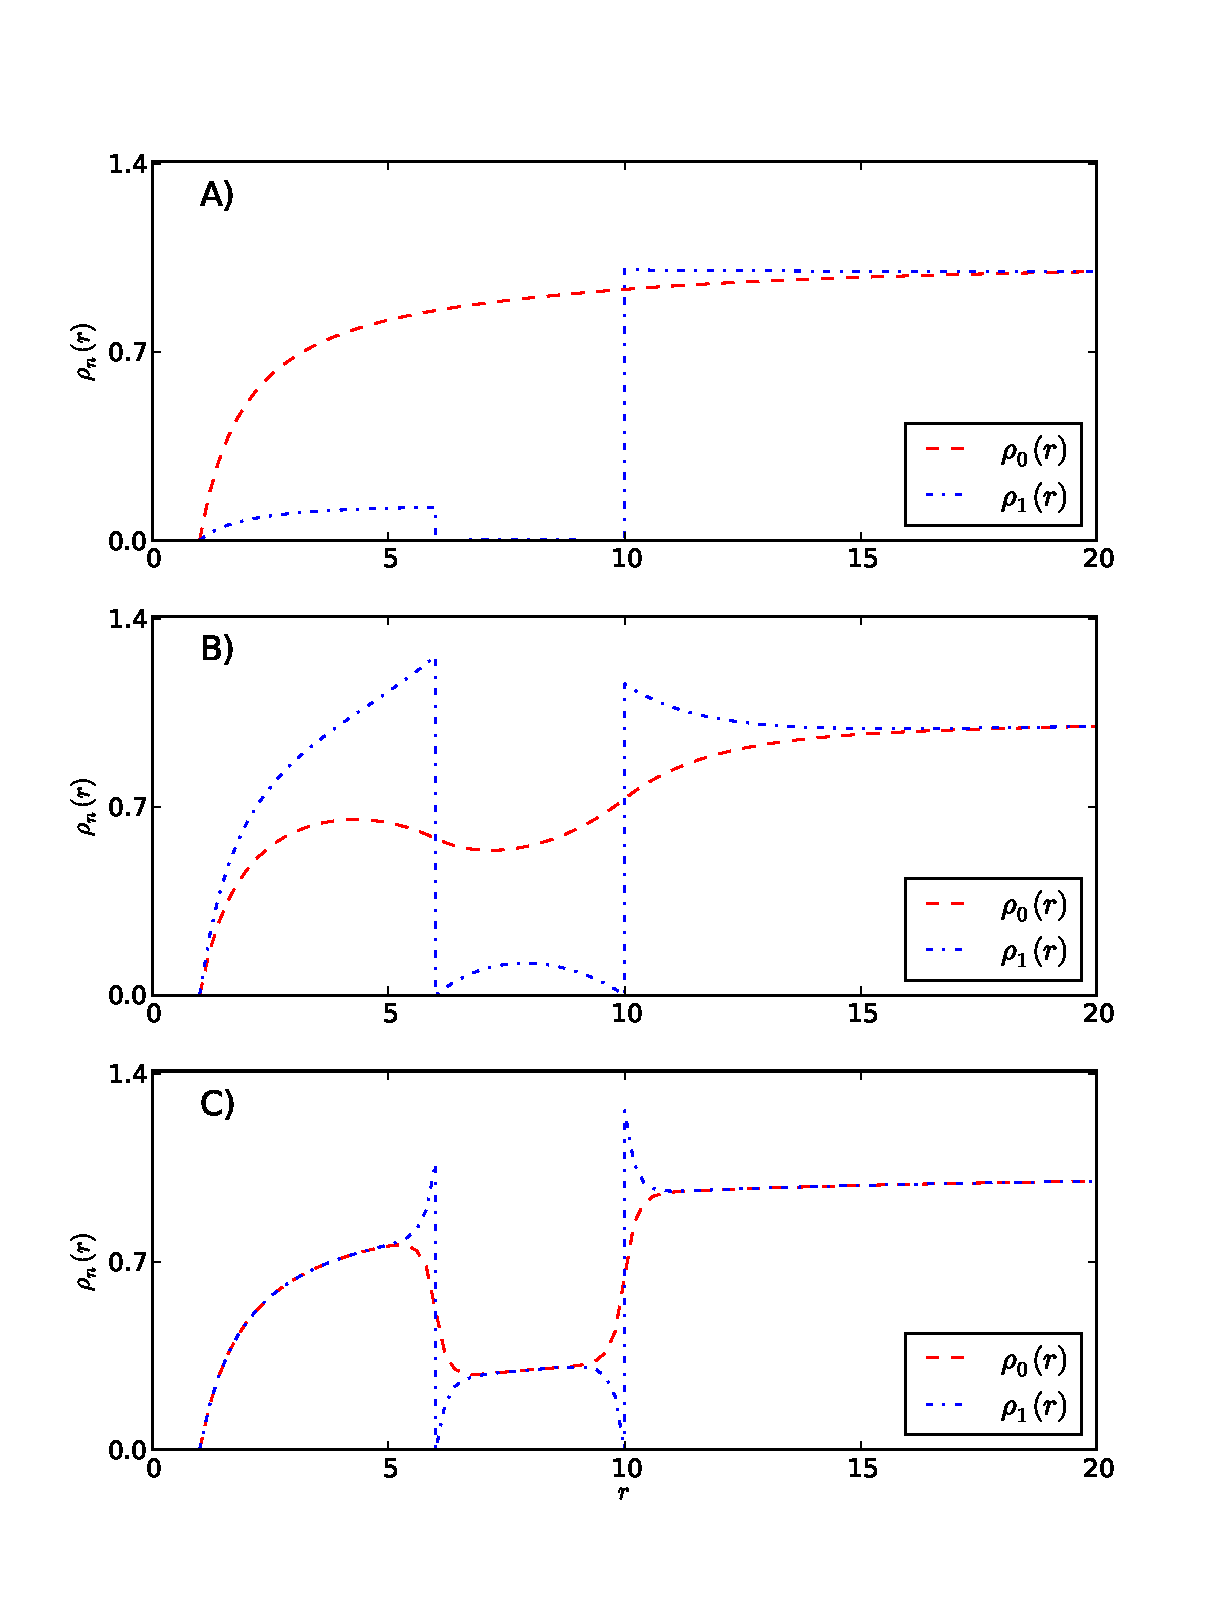
\includegraphics[width = 1 \textwidth]{plots/density_profiles.pdf}
        \end{tikzfigure}
        \vspace{-1.3 cm}
        \end{minipage}\begin{minipage}[t]{.57 \textwidth}
            \vspace{.5 cm}
            Examples of density profiles for symmetric $\gamma_{10}=\gamma_{01} = \gamma$ and attractive metastable barrier.
            \begin{itemize}
                \item The figure shows density profiles for the active $\rho_0(r)$ and inactive $\rho_1(r)$ state of the barrier, as well as the mean density profile.
                \item The three figures differ in the ratio of diffusion constant of the Brownian particles to the switching rate which influences the decay length of the influence of the potential (comp. eq. \eqref{fp_ind_sol})
            \end{itemize}
            \begin{equation}
                r_d = \sqrt{\frac{D}{\lambda_1}}=\sqrt{\frac{D}{2 \gamma}}
                \label{decay_length}
            \end{equation}
            \coloredbox{colorthree!60!}{Obviously, this decay length gives the radial range of the influence of the potential.}
            \vspace{-.3 cm}
            \begin{tikzfigure}[Density profiles for barrier with $U_0 = 0$, $U_1=10$, $l=5$ and $g=1$. A: $r_d = 25$, B: $R_d = 2.5$, C: $R_d= 0.25$]
            \end{tikzfigure}
        \end{minipage}
    }
    \blocknode{Absorption Rates - Resonant Activation}{
        \vspace{.4 cm}
        \begin{minipage}[t]{.48 \textwidth}
            \center
            \textbf{Attractive Barrier}
            \vspace{0.3 cm}
            \begin{tikzfigure}
            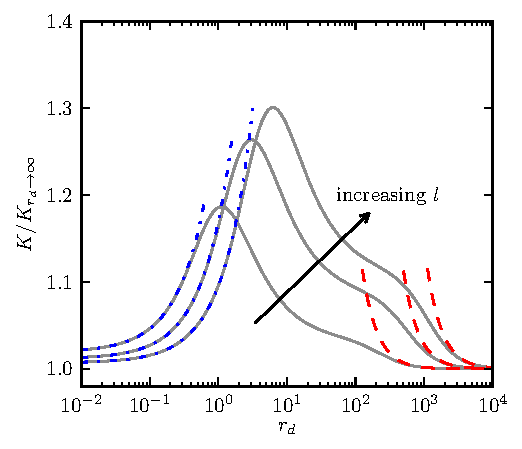
\includegraphics[width = 1 \textwidth]{plots/ab_rates.pdf}
            \end{tikzfigure}
        \end{minipage}\begin{minipage}[t]{.48 \textwidth}
            \center
            \textbf{Repulsive Barrier}
            \begin{tikzfigure}
                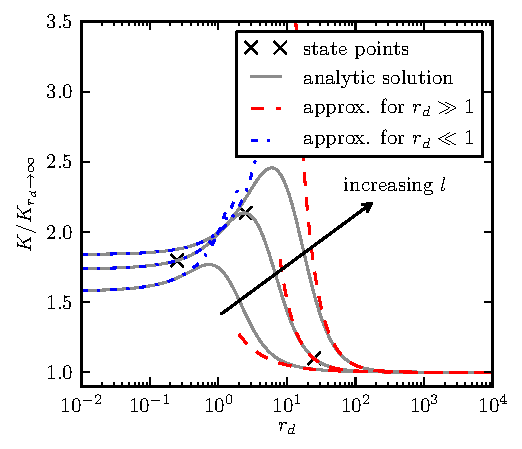
\includegraphics[width = 1 \textwidth]{plots/rb_rates.pdf}
            \end{tikzfigure}
        \end{minipage}
        \vspace{-.7 cm}
        \begin{tikzfigure}[normalized absorption rate vs. decay length for attractive fluctuating barrier. \newline Parameters are $U_1 = 10,-10 , U_0= 0, g = 1$ and $l=2,5,10$. ]
        
        \end{tikzfigure}
        \vspace{-.7cm}
        \hspace{0.019 \textwidth}\begin{minipage}[t]{.47 \textwidth}
            \coloredbox{colorthree!50!}{\textbf{Breathing Barrier} $U_1<0$: the barrier collects particles while at an active state and releases them when its state changes.}
        \end{minipage}\hspace{0.07 \textwidth}\begin{minipage}[t]{.42 \textwidth}
            \coloredbox{colorthree!50!}{\textbf{Pumping Barrier} $U_1>0$: particles can cross the outer barrier border while it is down and get lifted up when the barrier state changes.}
        \end{minipage}
        \vspace{.4 cm}
        \hspace{0.025 \textwidth}\begin{minipage}[t]{.48 \textwidth}
        The absorption rate profiles exhibit a resonant peak depending on decay length and size of the barrier. Similar phenomena are found in escape over fluctuating barriers. The resonant peak follows a power law: 
        \begin{equation}
            r_d^{(res)} = C l^{\kappa}
            \label{powerlaw}
        \end{equation}
        with $C \approx 1$ and $\kappa \approx 2/5$. Also for fixed gap to width ratio $g$ of the barrier, the resonant rate $K^{(res)}$ converges to a finite value.
        \begin{tikzfigure}[Resonant decay length $r_d^{(res)}$ and absorption rate $K^{(res)}$ for repulsive parrier $U_1 = 10$ and $g = 1$]
        \end{tikzfigure}
    \end{minipage}\hspace{0.05 \textwidth}\begin{minipage}[t]{.48 \textwidth}
        \vspace{-1 cm}
        \begin{tikzfigure}
           \hspace{-3 cm} 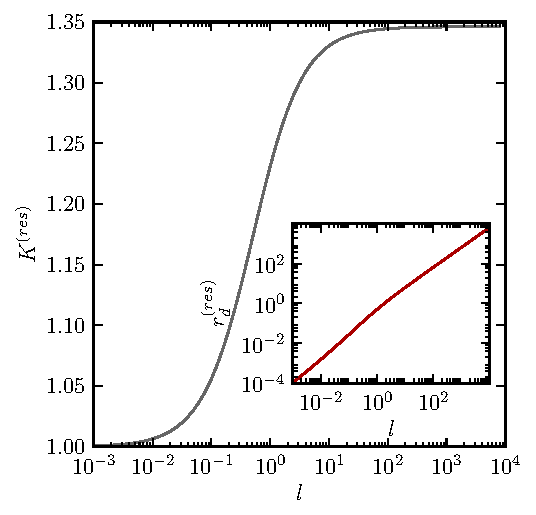
\includegraphics[width = .9 \textwidth]{plots/powerlaw.pdf}
        \end{tikzfigure}
    \end{minipage}

                }
    \blocknode{Limit $l \ll 1$ $\rightarrow$ No Resonant Activation}{
        \vspace{.5 cm}
        \hspace{0.005 \textwidth}\begin{minipage}[t]{.48 \textwidth}
        In the limit of $t \gtrsim 0$ the system can locally be approximated by a metastable barrier in front of an absorbing wall.
        \begin{tikzfigure}
            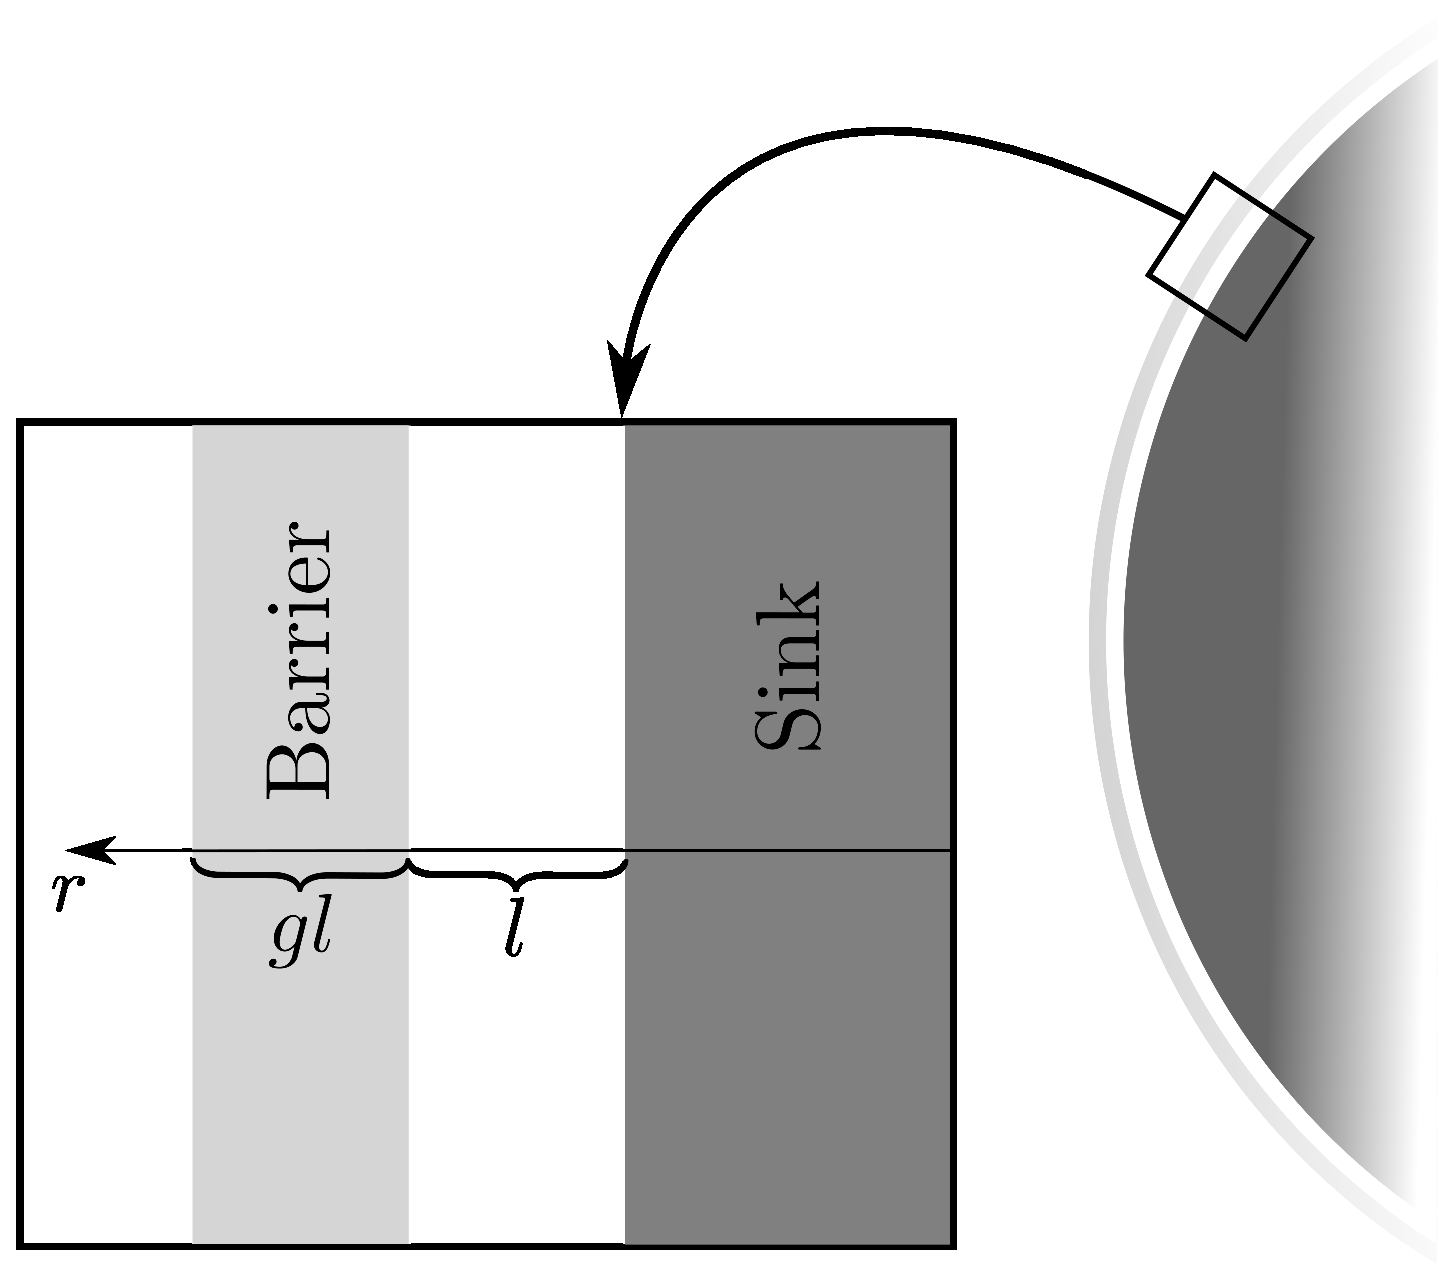
\includegraphics[width = 1 \textwidth]{plots/tlimit.eps}
        \end{tikzfigure}
        In this case, the problem is one dimensional on the microscopic level of a particle right at the potential barrier.
        \end{minipage}\hspace{0.02 \textwidth}\begin{minipage}[t]{.48 \textwidth}
        For the absorption rate there are three fundamentally different cases:
        \begin{itemize}
            \item The finite barrier $|U_1|<0$
        \end{itemize}
        \begin{equation}
            K \approx 4 \pi D \left(1 - \frac{1}{2}\left( e^{U_1}-1\right)gl + \mathcal{O}(l^{2})\right) \nonumber
        \end{equation}
        \begin{itemize}
            \item The ideal attractive barrier $U_1 \rightarrow - \infty$
        \end{itemize}
        \begin{equation}
            K \approx 4 \pi D \left( 1 + \frac{gl}{4} + \mathcal{O}(l^{2})\right) \nonumber
        \end{equation}
        \begin{itemize}
            \item The ideal repulsive barrier $U_1 \rightarrow \infty$
        \end{itemize}
        \begin{equation}
            K \approx 4 \pi D \left( \frac{1+r_d}{1 + 2 r_d} - \frac{(g+1)l}{(2r_d+1)^{2}} + \mathcal{O}(l^{2})\right) \nonumber
        \end{equation}
        All of these expressions have in common, that they do \textit{not have a maximum} but are either constant or in the last case interpolate monotonously between two values. \par
        \vspace{.5 cm}
        \coloredbox{colorthree!100!}{
             \textbf{The curvature of the potential barrier must therefore be a crucial criterion for resonant activation to take place.}}
    \end{minipage}
    \vspace{-.7 cm}
    }
\end{tikzpicture}
\end{document}
